% Copyright (c) 2024, Francisco Fernandez
% License: CC BY-SA 4.0
%   https://github.com/fernandezfran/thesis/blob/main/LICENSE
\chapter{Métodos computacionales}\label{ch:metodos}
\thispagestyle{empty}

\vspace{50pt}

\begin{adjustwidth}{50pt}{50pt}
    En este capítulo se introducen las técnicas de simulación computacional que se utilizan
    en esta tesis. Esta incluye distintas escalas espaciales y temporales, por 
    lo que se introducen tanto modelos atomísticos como modelos del continuo.
    Además, se mencionan los softwares que se utilizaron/implementaron a lo largo
    de la tesis.
\end{adjustwidth}

\clearpage
\newpage
\thispagestyle{empty}
\mbox{}
\newpage

% Copyright (c) 2024, Francisco Fernandez
% License: CC BY-SA 4.0
%   https://github.com/fernandezfran/thesis/blob/main/LICENSE
\section{Técnicas de simulación a distintas escalas}

Dentro de la física, la química y las ciencias de los materiales existen diversas
técnicas computacionales para desarrollar modelos capaces de predecir y entender 
las propiedades de algún sistema en particular. Estos modelos no son más que 
abstracciones matemáticas o lógicas de la realidad que permiten obtener dicha 
información de interés a costa de renunciar a otra \cite{franco2013}. 
En la Figura \ref{fig:escalas} se muestran aplicaciones específicas de 
simulaciones numéricas que cubren distintos intervalos de escalas espaciales y 
temporales. Con respecto a las baterías de litio, se han estudiado distintas
componentes de las mismas con técnicas tales como DFT \cite{he2019}, Dinámica 
molecular \cite{yao2022}, Monte Carlo \cite{mercer2017}, Monte Carlo cinético 
\cite{gavilan2021}, Dinámica mesoescala \cite{ryan2019} y Modelos del continuo
\cite{brosa2022}. En particular, en esta tesis se utilizan las técnicas 
resaltadas con colores en la Figura \ref{fig:escalas} para estudiar distintos 
aspectos de materiales de interés en el área de las baterías de ion-litio.
\begin{figure}[h!]
    \centering
    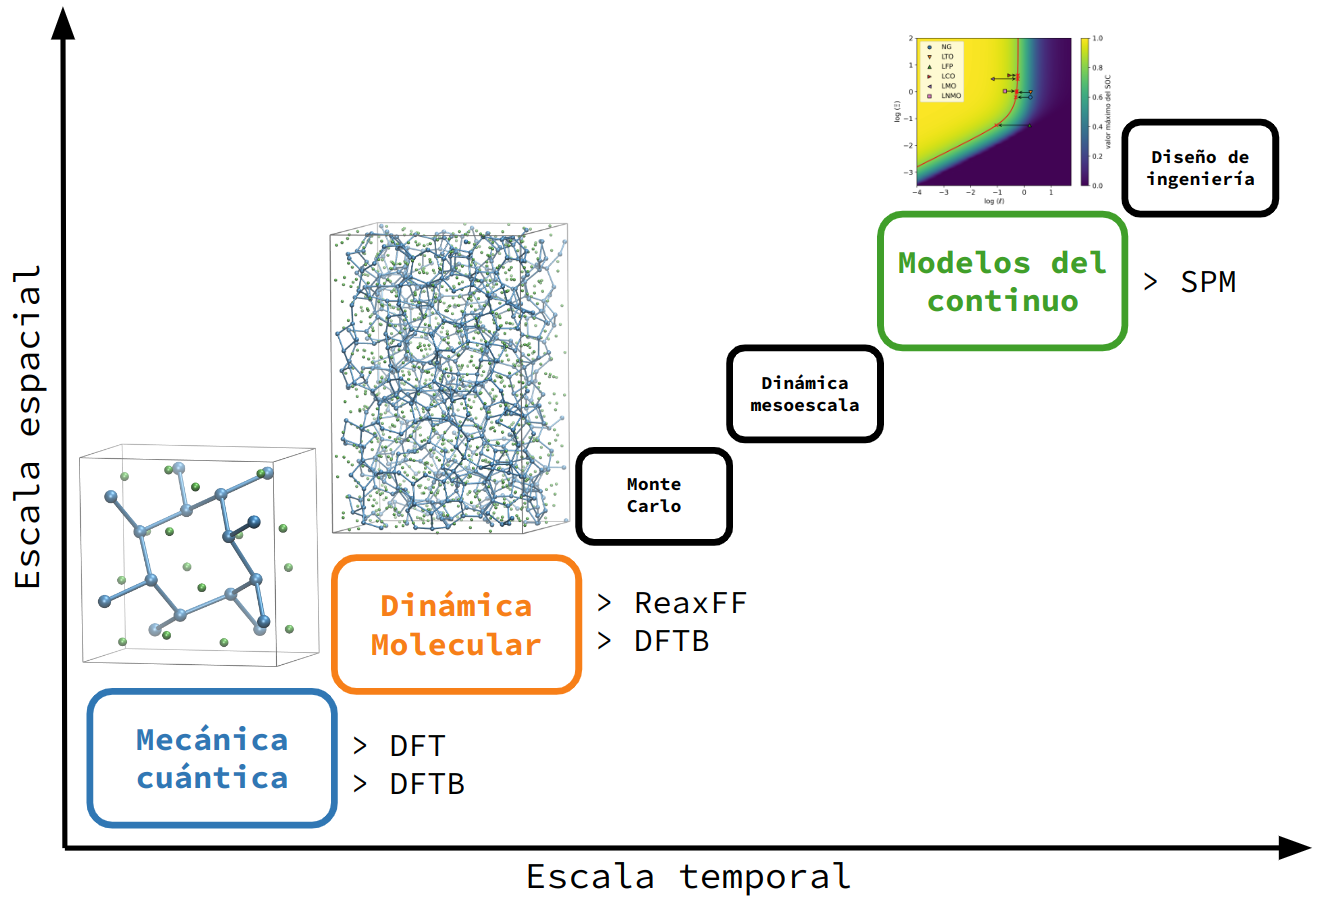
\includegraphics[width=.8\textwidth]{Metodos/tecnicas/escalas.png}
    \caption{Esquema de escalas espaciales y temporales relativas de distintas 
    técnicas de simulaciones computacionales. Se destacan con colores aquellas que 
    se utilizaron en esta tesis mientras que se mencionan otras.}
    \label{fig:escalas}
\end{figure}

Los métodos tradicionales de prueba y error requieren demasiado tiempo como 
para seguir el ritmo rápido de crecimiento en la demanda de sistemas de 
almacenamiento y transporte de energía. %, que actualmente se encuentran limitados por los materiales disponibles. 
Esto ha atraído la atención de investigadores e ingenieros 
hacia el desarrollo de modelos computacionales, desde la escala atómica hasta la 
escala del continuo, y la integración de las mismas, para tener una herramienta 
predictiva para resolver los problemas relacionados a los electrones, los átomos, 
los clusters, las partículas, los electrodos, las celdas e incluso el pack de 
baterías \cite{shi2016}. En particular, en la escala atómica usualmente se tienen
predicciones bajo equilibrio termodinámico de propiedades como la estructura, 
transformaciones de fase, energías de activación, entre otras, como se lo realiza
en la Parte \ref{p:silicio} de esta tesis para el caso de los ánodos de silicio. 
Además de esto, se busca encontrar relaciones que mapeen dichas propiedades con 
descriptores más simples de obtener \cite{juan2021}, como se propone en la Parte
\ref{p:fast-charging} de esta tesis al ajustar datos experimentales con un modelo
del continuo.

Como perspectiva futura, las técnicas de simulación a distintas escalas 
mencionadas aquí pueden combinarse para desarrollar modelos multi-escala 
\cite{franco2019}, y a su vez también pueden aplicarse métodos de inteligencia 
artificial/aprendizaje automático \cite{lombardo2021}, con el objetivo diseñar y 
optimizar las baterías de litio de próxima generación. 


% Copyright (c) 2024, Francisco Fernandez
% License: CC BY-SA 4.0
%   https://github.com/fernandezfran/thesis/blob/main/LICENSE
\section{Modelos atomísticos}\label{s:atomicos}

\subsection{Teoría del funcional de la densidad (DFT)}

El desarrollo de la mecánica cuántica, y las observaciones experimentales que la
validan, fue uno de los avances científicos más significativos del siglo veinte. 
Esta teoría permite estudiar cómo varía la energía de los materiales con el 
movimiento de los átomos. Esto gracias a la aproximación de Born-Oppenheimer, que 
separa el movimiento de los núcleos del de los electrones al considerar que los primeros son mucho más
pesados que los segundos. Esto implica que se puede considerar que los electrones 
responden mucho más rápido a los cambios en su entorno que los núcleos, lo que 
permite resolver las ecuaciones que describen su movimiento fijando las 
posiciones de los núcleos atómicos. Así se encuentra el estado fundamental de los
electrones, es decir, su configuración de menor energía \cite{shankar2012}.

La ecuación de Schrödinger no-relativista e independiente del tiempo,
\begin{equation}\label{eq:schrodinger}
    H \psi = E \psi,
\end{equation}
caracteriza un sistema físico desde un enfoque cuántico, donde $\psi$ es un
conjunto de soluciones, o autoestados, del Hamiltoniano $H$ que tienen asociados los
autovalores $E$ que satisfacen dicha ecuación. 
%Para el caso en el que se desee estudiar
%la interacción entre varios electrones y núcleos una descripción más completa de la 
%ecuación de Schrödinger es la siguiente,
%\begin{equation}\label{eq:schrodinger}
%    \left[ - \frac{\hbar^2}{2 m} \sum_{i=1}^N \nabla_i^2 + \sum_{i=1}^N V(\mathbf{r}_i) + \sum_{i=1}^N \sum_{i<j} U(\mathbf{r}_i, \mathbf{r}_j) \right] \psi = E \psi,
%\end{equation}
%donde $\hbar$ es la constante de Planck reducida, $m$ la masa del electrón, el primer 
%término describe la energía cinética de cada electrón, el segundo la energía de 
%interacción de cada electrón con todos los núcleos y el tercero la energía de 
%interacción entre distintos electrones. Este último término es el más crítico desde 
%el punto de vista de la resolución de la ecuación.

%Ahora, la cantidad que puede medirse es la probabilidad de que los $N$ electrones 
La cantidad que puede medirse es la probabilidad de que los $N$ electrones 
estén en un conjunto de posiciones $\lbrace \mathbf{r}_i \rbrace$ en cualquier orden. 
Una cantidad relacionada a dicha probabilidad es la densidad de electrones,
$n(\mathbf{r})$. Esta se puede escribir como 
\begin{equation}
    n(\mathbf{r}) = 2 \sum_i \psi_i^*(\mathbf{r}) \psi_i(\mathbf{r}),
\end{equation}
donde la suma se realiza sobre todos los electrones $i$ y el producto de $\psi_i$ con su 
complejo conjugado $\psi_i^*$ es el cálculo de la probabilidad asociada al electrón $i$. 
Lo destacable de esta ecuación es que reduce la solución completa de la función de onda
de la ecuación de Schrödinger de $3 N$ coordenadas a tan sólo 3 y, además, contiene una 
gran cantidad de información que es observable, $n(\mathbf{r})$.

La teoría del funcional de la densidad electrónica (DFT por sus siglas en inglés
\textit{Density functional theory}) es un método altamente efectivo para 
encontrar soluciones a la ecuación fundamental que describe el comportamiento 
cuántico de átomos y moléculas en sistemas de materia condensada, la ecuación 
\ref{eq:schrodinger} de Schrödinger, en situaciones de utilidad práctica 
\cite{sholl2022}. La misma se basa en dos teoremas matemáticos fundamentales
demostrados por Hohenberg y Kohn \cite{hohenberg1964} y la derivación de un 
conjunto de ecuaciones realizada por Kohn y Sham \cite{kohn1965}.

El primero de los teoremas establece: \say{La energía del estado fundamental 
de la ecuación de Schrödinger es un funcional unívoco de la densidad
electrónica}, es decir que la energía $E$ puede expresarse como 
$E[n(\mathbf{r})]$.

El segundo teorema define la siguiente propiedad: \say{La densidad electrónica
que minimiza la energía del funcional global es la densidad verdadera de los 
electrones correspondiente a la solución completa de la ecuación de Schrödinger}.
Si se conociera la forma del funcional \say{verdadera} podría variarse la 
densidad electrónica hasta que se minimice su energía, este es el principio 
variacional y en la práctica se lo utiliza con formas aproximadas del funcional.

Al funcional de la energía se lo puede plantear en dos términos,
\begin{equation}
    E[\lbrace \psi_i \rbrace] = E_{\text{conocido}}[\lbrace \psi_i \rbrace] + E_{\text{XC}}[\lbrace \psi_i \rbrace].
\end{equation}
El primero de ellos involucra cuatro contribuciones que pueden expresarse 
analíticamente: la energía cinética del electrón y las interacciones de tipo 
Coulomb (electrón-núcleo, electrón-electrón y núcleo-núcleo), mientras que
el segundo de los términos es el funcional de la correlación de intercambio
que se define para incluir todos los efectos mecánico cuánticos que no estén
incluidos en los términos \say{conocidos}. Kohn y Sham demostraron que la 
solución de la ecuación puede plantearse en términos de la función de onda 
de un sólo electrón que depende de tres variables espaciales.

De la \say{derivada} del funcional de la correlación de intercambio puede 
definirse el potencial de correlación de intercambio como sigue
\begin{equation}
    V_{\text{XC}}(\mathbf{r}) = \frac{\delta E_{\text{XC}}(\mathbf{r})}{\delta n(\mathbf{r})}.
\end{equation}
La solución exacta de la densidad electrónica ha sido demostrada para un gas 
uniforme de electrones. Luego, una aproximación local de la densidad (LDA,
\textit{local density aproximation}) utiliza la densidad local para definir 
un potencial de correlación de intercambio aproximado,
\begin{equation}
    V_{\text{XC}}(\mathbf{r}) = V_{\text{XC}}^{\text{gas de electrones}}[n(\mathbf{r})].
\end{equation}
Otras aproximaciones también utilizan información del gradiente local en 
la densidad electrónica, lo cual define la aproximación generalizada del 
gradiente (GGA, \textit{generalized gradient approximation}). Uno de los
funcionales más utilizados para sólidos es el de Perdew-Burke-Ernzerhof (PBE).


\subsection{Funcional de la densidad de enlace fuerte (DFTB)}\label{s:dftb}

El formalismo del funcional de densidad de enlace fuerte (DFTB, \textit{density
functional tight-binging}) ha sido ampliamente descripto en la literatura 
\cite{elstner1998,frauenheim2000,seifert2007,gaus2011}. El método DFTB se basa 
en una expansión a segundo orden de la energía de la teoría del funcional de la 
densidad (DFT) con respecto a una fluctuación de la densidad electrónica de 
referencia \cite{foulkes1989}. La energía de DFTB resultante puede escribirse de 
la siguiente manera:
\begin{equation}\label{eq:dftb}
    E_{\text{DFTB}}=\sum_i^{\text{occ}}\langle\psi_i|\hat{H}^0|\psi_i\rangle+\frac{1}{2}\sum_{AB}\gamma_{AB}\Delta q_A\Delta q_B+E_{\text{rep}}^{AB}
\end{equation}
donde $\psi_i$ denota los orbitales Kohn-Sham (KS) de una partícula. Con una 
combinación lineal de orbitales atómicos, $\psi_i$ se expande en un conjunto de 
orbitales de valencia pseudoatómicos de tipo Slater $\phi_\nu$,
\begin{equation}
    \psi_i({\bf r})=\sum_\nu c_{\nu i}\phi_\nu({\bf r}-{\bf r}_A),
\end{equation}
que se determinan resolviendo la ecuación secular KS
\begin{equation}\label{eq:ks}
    \sum_\mu c_{\mu i}\left(H^0_{\nu\mu}-\epsilon_iS_{\nu\mu}\right)=0, \;\;\forall \nu,i
\end{equation}
donde $S_{\nu\mu}=\langle \phi_\nu| \phi_\mu\rangle$ y $\epsilon_\nu$ son la 
matriz de superposición y los autovalores de un átomo aislado, respectivamente.
${H}^0_{\nu\mu}$ es el Hamiltoniano efectivo KS generado con la densidad 
electrónica de referencia, $\rho^0$, y está definido como
\begin{equation}\label{eq:h0}
    H^0_{\nu\mu}=\begin{cases}
        \epsilon_\mu & \text{si}\; \nu=\mu\\
        \langle \phi_{\nu}| -\frac{1}{2}\nabla^2+v_{\text{eff}}\left[\rho_A^0+\rho_B^0\right]|\phi_{\nu}\rangle&\text{si}\;\mu\in A,\; \nu\in B\;\text{y} \;A\ne B\\
        0& \text{si no}
    \end{cases}
\end{equation}
donde $\rho_A^0$ es la densidad de referencia de un átomo neutro $A$ y 
$v_{\text{eff}}$ el potencial KS efectivo, construido a partir de la superposición
de densidades centradas en átomos neutros. En particular, los elementos de la 
matriz del Hamiltoniano dependen solo de los átomos $A$ y $B$, por lo tanto sólo
se calculan explícitamente los elementos de dos centros de las matrices del 
Hamiltoniano y de superposición en función de la distancia y la orientación, usando 
las reglas de transformación de Slater-Koster \cite{slater1954}.

Una de las partes cruciales del uso del método DFTB es calcular las funciones 
base y las densidades atómicas $\phi$ y $\rho^0$, respectivamente. Los orbitales
pseudoatómicos y las densidades se obtienen de resolver las ecuaciones atómicas KS 
modificadas en las que se agrega un potencial de confinamiento, $V_{\text{conf}}$,
\begin{equation}\label{eq:dft}
    \left[\hat{T}+V_{\text{eff}}+V_{\text{conf}}\right]\phi_\mu=\epsilon_\mu\phi_\mu.
\end{equation}
Una práctica común dentro de la comunidad de DFTB consiste en elegir un potencial
de confinamiento parabólico, cuadrático, o una función de ley de potencia.

El segundo término en la ecuación \ref{eq:dftb} es la energía debida a las 
fluctuaciones de cargas y se parametriza analíticamente como una función de las
cargas orbitales y de $\gamma_{AB}$, que a su vez es una función de la separación 
interatómica y del parámetro de Hubbard, $U$, que se obtienen suponiendo que son 
iguales a los de los átomos aislados y se calculan como la diferencia de la 
afinidad electrónica y la energía de ionización para distintos momentos angulares 
orbitales \cite{elstner1998b}. $\Delta q_X = q_X - q_X^0$ es la carga de Mulliken 
inducida autoconsistente en el átomo $X$ \cite{elstner1998}.

La contribución restante a la energía total de DFTB en la ecuación \ref{eq:dftb}
es $E_{\text{rep}}$ y se corresponde con el potencial repulsivo diatómico que 
depende de la distancia y contiene los efectos de los electrones del núcleo, los 
términos de repulsión ion-ion y efectos de intercambio-correlación. 
La energía total repulsiva de un sistema es una suma de contribuciones de 
potenciales repulsivos $V_{\text{rep}}(r)$ de cada par de átomos
\begin{equation}\label{eq:rep}
    E_{\text{rep}}=\sum_{i<j} V_{\text{rep}}(r_{ij})
\end{equation}
donde $i$ y $j$ son los índices de los átomos en el sistema y $r_{ij}$ es la 
distancia entre ellos. Generalmente se considera que $V_{\text{rep}}$ es una
función empírica que se determina al ajustar datos de cálculos de estructura 
electrónica de un nivel superior, como DFT.


\subsection{Dinámica molecular}

En la mayoría de los experimentos que se realizan en un laboratorio se obtiene 
una serie de mediciones sobre sistemas macroscópicos, usualmente constituidos por 
más de 10$^{20}$ moléculas, durante un período de tiempo, a las cuales luego se 
les realiza un promedio. La mecánica estadística ofrece una interpretación de 
las propiedades del equilibrio de sistemas macroscópicos a partir de una teoría 
molecular aplicada a su configuración microscópica ~\cite{hill1986}.

Esta teoría relaciona el promedio temporal de una variable mecánica con el 
promedio de ensambles, donde un ensamble es una colección de un número muy largo
de sistemas construidos de manera tal que reproducen las propiedades 
termodinámicas del sistema en cuestión a partir de sus configuraciones atómicas
\cite{salinas2001}. Esto es el primer postulado de la Mecánica estadística y se 
lo conoce como la \textit{hipótesis ergódica}: \say{El promedio temporal de una 
variable mecánica $M$ en el sistema termodinámico de interés es igual al promedio 
de ensambles de $M$, en el límite del conjunto de ensambles que tiende a infinito, 
siempre que los sistemas del conjunto de ensambles reproduzcan el estado 
termodinámico y el entorno del sistema real de interés}. Para poder aplicar
este postulado se necesita conocer la probabilidad relativa de cada uno de los 
estados presentes en el ensamble. A esto se refiere el segundo postulado de la 
Mecánica estadística de \textit{igual probabilidad a priori}: \say{En un conjunto 
de ensambles representativo de un sistema termodinámico aislado, los sistemas del 
conjunto de ensambles se distribuyen uniformemente, es decir, con igual 
probabilidad o frecuencia, sobre los posibles estados con los valores
especificados de dicho sistema termodinámico aislado}. En otras palabras, cada 
estado está representado por la misma cantidad de sistemas en el ensamble.

Cuando las \textit{fluctuaciones} son pequeñas, la función de distribución de 
probabilidad de la variable mecánica $M$ tiene una forma gaussiana en torno a su 
valor medio $\overline{M}$, por lo que su dispersión puede caracterizarse 
completamente por su desviación estándar $\sigma_M$, es decir,
\begin{equation}
    \sigma_M = \sqrt{\overline{(M - \overline{M})^2}}.
\end{equation}
Puede demostrarse que las \textit{fluctuaciones} de la variable mecánica $M$ 
decrecen a medida que aumenta el número de partículas $N$ presentes en el sistema 
de forma proporcional a la inversa de su raíz,
\begin{equation}\label{eq:fluctuaciones}
    \frac{\sigma_M}{\overline{M}} \approx \mathcal{O}(N^{-1/2}).
\end{equation}

Las simulaciones de Dinámica Molecular (MD, de sus siglas en inglés, 
\textit{Molecular Dynamics}) consideran un sistema clásico de muchos cuerpos 
interactuantes bajo un campo de fuerzas newtoniano para estudiar propiedades de 
equilibrio y transporte. Dada la configuración de $N$ partículas se tiene el 
siguiente sistema de ecuaciones de Newton por resolver
\begin{equation}
    m_i \frac{\partial^2 \mathbf{r}_i}{\partial t^2} = \mathbf{F}_i, \quad i = 1,..., N,
\end{equation}
donde $m_i$ es la masa del átomo $i$, $\mathbf{r}_i$ su posición y $\mathbf{F}_i$
la fuerza. Estas ecuaciones de movimiento son integradas en intervalos de tiempo
pequeños que permiten obtener la evolución temporal del sistema, es decir, su
trayectoria. Ya introducida la mecánica estadística, pueden extraerse propiedades
macroscópicas del sistema en equilibrio al considerar configuraciones microscópicas
representativas a distintos instantes de tiempo de la trayectoria
\cite{allen2017, frenkel2001}.

En la Figura \ref{fig:esquema_md} se muestra un diagrama de flujo de un algoritmo
típico de dinámica molecular para entender el funcionamiento de esta técnica de 
simulación. El mismo está conformado por las siguientes partes:
\begin{figure}[h!]
    \centering
    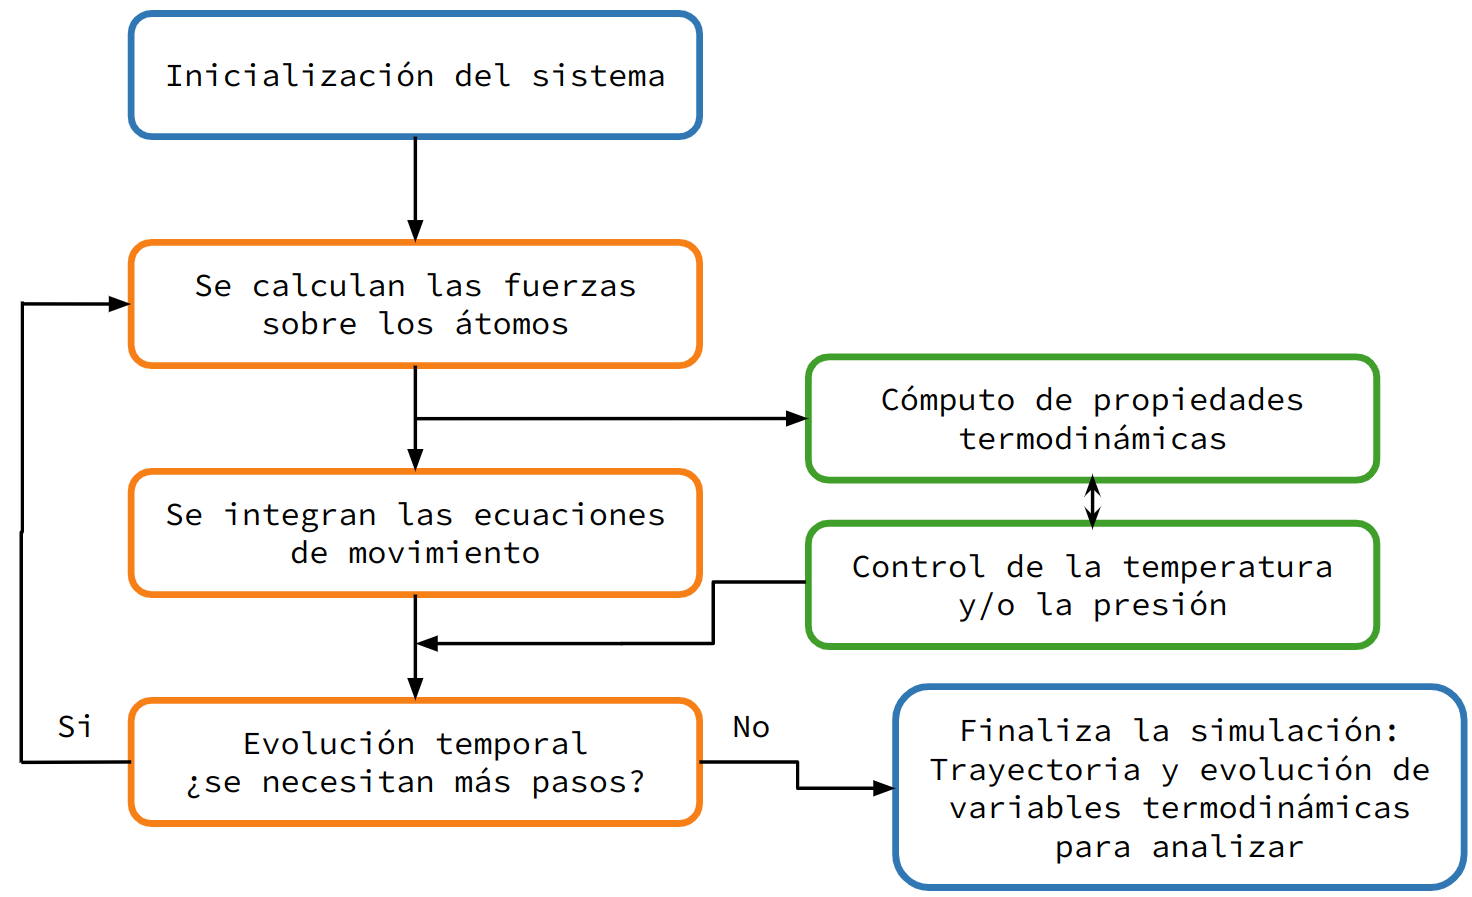
\includegraphics[width=\textwidth]{Metodos/atomicos/esquema.png}
    \caption{Esquema de un diagrama de flujo de una dinámica molecular usual.}
    \label{fig:esquema_md}
\end{figure}
\begin{enumerate}
    \item \textbf{Inicialización del sistema}: se especifican las posiciones y
        velocidades iniciales de los átomos, el tamaño y la forma de la celda de 
        simulación. También se elije un paso temporal y las condiciones de 
        contorno.
    \item \textbf{Campo de fuerzas}: con el sistema inicializado se calcula la 
        fuerza sobre cada uno de los átomos.
    \item \textbf{Cómputo de propiedades termodinámicas}: se realizan los
        cálculos de distintas cantidades de interés, como las energías potencial
        y cinética, la presión y la temperatura, etc.
    \item \textbf{Integración de las ecuaciones de movimiento}: se integran las
        ecuaciones de Newton mediante algún integrador que obtiene las posiciones
        y velocidades del paso temporal siguiente a partir del actual.
    \item \textbf{Control de la temperatura y/o la presión}: para que la 
        simulación se realice en el ensamble termodinámico deseado.
    \item \textbf{Evolución temporal}: se incrementa el tiempo adicionando un
        paso temporal y se vuelve a realizar el cálculo de las fuerzas sobre las 
        nuevas configuraciones hasta alcanzar el número de pasos temporales 
        deseados.
\end{enumerate}
Luego de este proceso se tiene la evolución temporal de las distintas propiedades
termodinámicas de interés y la trayectoria del sistema para ser analizada 
posteriormente, por ejemplo con los observables que se definirán en la sección 
\ref{s:observables}. A continuación se dan más detalles sobre cada uno de los 
pasos mencionados.


\subsubsection{Inicialización del sistema}

Existe una base de datos, Materials Project \cite{materials_project}, 
ampliamente utilizada en el ámbito académico y en la industria que 
recopila estructuras optimizadas con DFT, realiza nuevos cálculos y 
está abierta a la comunidad para su uso y colaboración. Antes de que 
los datos se carguen en la página, los mismos son comparados con resultados 
experimentales para determinar si están dentro de un rango de validez definido. 
En esta tesis en particular, se utilizaron distintas estructuras cristalinas de 
esta base de datos como condiciones iniciales para las posiciones y los tamaños 
de las celdas de simulación.

Las velocidades de los átomos suelen ser generadas de manera aleatoria, a través
de un generador de números pseudo-aleatorio, tomando como argumento una semilla 
para la reproducibilidad de la simulación y una temperatura deseada para el
sistema. Estos números son generados con una distribución gaussiana, donde el 
centro se lo fija a cero para que no haya una velocidad en el centro de masa y 
el ancho está relacionado a la temperatura seleccionada.

Además de dar la configuración inicial de los átomos, es necesario especificar si
los mismos se encuentran dentro de una celda de simulación con un tamaño en
particular para cada una de las direcciones del sistema o si no interactúan fuera
del borde de la estructura que conforman los mismos. En el primero de los casos
se tienen condiciones periódicas de contorno (PBC, por sus siglas en inglés, 
\textit{periodic boundary conditions}), que busca reproducir un sistema infinito,
para que no existan efectos de borde, y consiste en considerar que los átomos se 
encuentran dentro de una celda unidad de una red infinita de celdas idénticas; en
donde si un átomo sale por un extremo de la celda, ingresa por el opuesto. % Una condición que debe cumplir esta celda es que su tamaño en cada una de las direcciones debe ser mayor al radio de corte de las interacciones entre los átomos. Por otro lado, el segundo de los casos es útil considerarlo cuando se tienen nanoestructuras en las cuales los átomos están ordenados de cierta forma que globalmente representan una forma definida y no pueden ser consideradas como una red infinita.


\subsubsection{Campo de fuerzas}

Los potenciales interatómicos empíricos o semi-empíricos que usualmente se 
utilizan en las simulaciones de MD relacionan la fuerza sobre un átomo con el 
entorno del mismo a través de una forma funcional conocida. Existe una gran 
variedad de estos potenciales y la elección de uno de ellos depende del sistema 
de estudio, ya que algunos potenciales representan de mejor manera gases y otros 
metales, por ejemplo. El potencial de Coulomb \cite{coulomb} considera las 
partículas como cargas puntuales que interactúan electrostáticamente. Los 
potenciales de Tersoff \cite{tersoff} o de Stillinger-Weber 
\cite{stillinger-weber} se desarrollaron especialmente para el modelado de 
materiales con enlaces covalentes fuertes. %, como es el caso del carbono o del silicio. 
El método del átomo embebido (EAM, de sus siglas en inglés) \cite{eam} 
y el EAM modificado (MEAM) \cite{meam} están diseñados para simular sistemas 
metálicos. Otros potenciales con enfoques más avanzados permiten simular
reacciones químicas en algunos sistemas, como es el caso de el COMB 
(\textit{charge-optimized many-body}) \cite{comb}, que incorpora una 
equilibración de las cargas en el modelo, o el del ReaxFF (\textit{reactive 
force fields}) \cite{reaxff}, que combina en un solo modelo distintas 
componentes de las que fueron mencionadas. En el último tiempo también se han 
desarrollado potenciales interatómicos de aprendizaje automático 
\cite{behler2016, behler2017, deringer2019}, que no tienen una forma funcional con
una interpretación física, si no más bien un mapeo entre las posiciones y la 
fuerza o la energía de un cálculo de un nivel más complejo, como puede ser DFT.

Para calcular la fuerza que actúa sobre el átomo $i$ se utiliza el opuesto 
de la derivada del potencial,
\begin{equation}\label{eq:fuerzas}
    \mathbf{F}_i = - \frac{\partial V}{\partial \mathbf{r}_i}.
\end{equation}

Para entender el comportamiento de los campos de fuerza se considera como ejemplo 
representativo el potencial de a pares de Lennard-Jones \cite{lennard-jones}, 
debido a que tiene una expresión simple de analizar,
\begin{equation}
    V_{LJ} = 4\varepsilon \left[ \left( \frac{\sigma}{r} \right)^{12} - \left( \frac{\sigma}{r} \right)^{6} \right],
\end{equation}
donde $r$ es la distancia entre dos átomos, $\varepsilon$ indica la profundidad 
del pozo del potencial que se encuentra en $r_m = 2^{1/6} \sigma$ y $\sigma$ es el
radio del átomo. En la figura \ref{fig:lj} se muestra el comportamiento de este
potencial, si la distancia entre dos átomos es menor a $r_m$ entonces se repelen,
si es mayor a dicha distancia, se atraen. Cuando la distancia entre dos átomos es 
infinita, los mismos no interactúan, en el caso práctico se define una distancia 
de corte, conocida como el \textit{radio de corte}, $r_{\text{cut}}$, a partir de 
la cual se considera que el potencial es nulo. Para evitar discontinuidades en 
este punto se suelen utilizar distintas técnicas como el truncado y desplazado o 
se multiplica al potencial alrededor de dicho punto por una función suave, que 
hace que el potencial se iguale suavemente a cero.
\begin{figure}[h!]
    \centering
    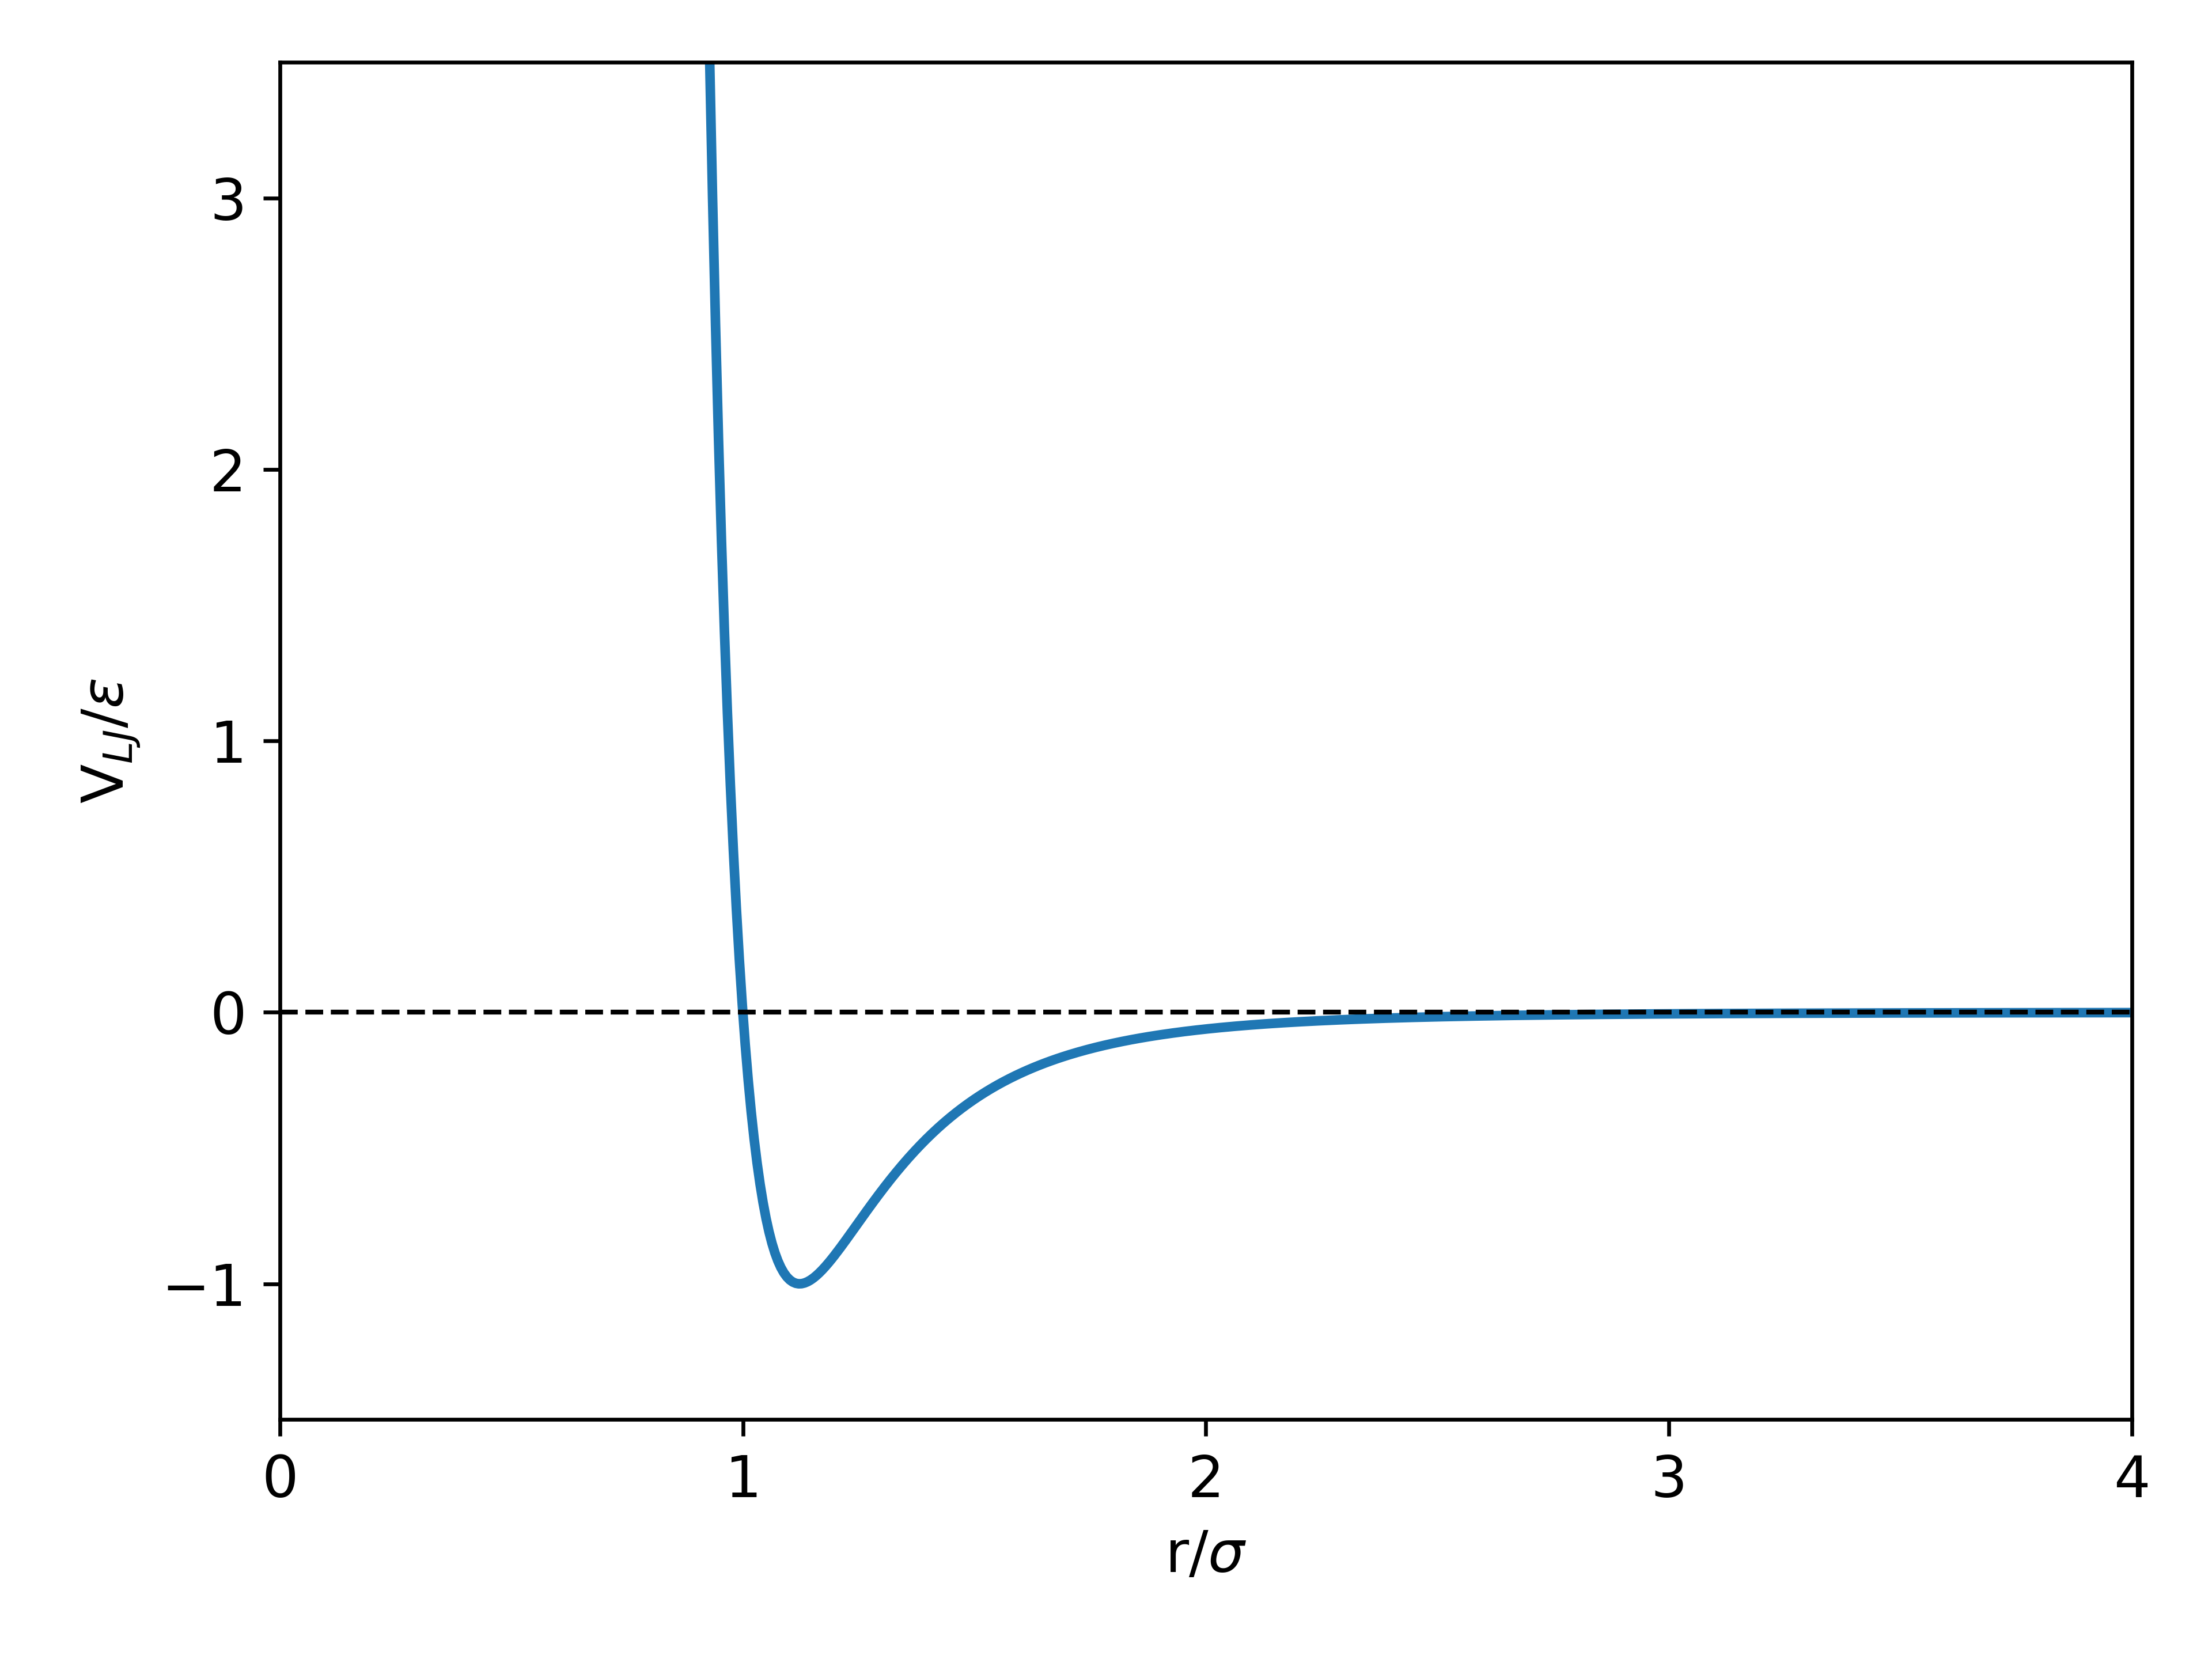
\includegraphics[width=0.7\textwidth]{Metodos/atomicos/lj.png}
    \caption{Gráfico de un potencial de Lennard-Jones en unidades reducidas.}
    \label{fig:lj}
\end{figure}

El ReaxFF \cite{reaxff} es el potencial reactivo del estado del arte para 
utilizar en simulaciones de MD de sistemas de interés en baterías de litio, ya
que representa adecuadamente la asociación y disociación de enlaces de átomos al 
considerar que la energía del sistema, $E_{\text{system}}$, se encuentra dividida
en varias contribuciones de energías parciales,
\begin{equation}\label{eq:reaxff}
    E_{\text{system}} = E_{\text{bond}} + E_{\text{over}} + E_{\text{under}} + E_{\text{val}} + E_{\text{pen}} + E_{\text{tors}} + E_{\text{conj}} + E_{\text{vdWaals}} + E_{\text{Coulomb}}.
\end{equation}
Una de las suposiciones fundamentales del ReaxFF es que el orden de enlace entre
un par de átomos puede obtenerse directamente de la distancia que los separa, 
esto se asegura con el término $E_{\text{bond}}$. $E_{\text{over}}$ y 
$E_{\text{under}}$ se agregan para imponer penalidades a los átomos 
sobrecoordinados o subcoordinados, utilizando la teoría de la valencia del enlace.
$E_{\text{val}}$ considera la contribución a la energía por el ángulo de valencia, 
mientras que $E_{\text{pen}}$ penaliza sistemas para reproducir la estabilidad de 
sistemas con dos dobles enlaces que comparten un átomo en un ángulo de valencia.
Las contribuciones a la energía de los ángulos de torsión y de los efectos de 
conjugación están dados por $E_{\text{tors}}$ y $E_{\text{conj}}$, 
respectivamente. Por último, las interacciones repulsivas a distancias 
interatómicas cortas y las atractivas a distancias largas son incluidas para 
todos los pares de átomos mediante un término de van der Waals, 
$E_{\text{vdWaals}}$, utilizando un potencial de Morse, y uno de Coulomb, 
$E_{\text{Coulomb}}$, donde las cargas de los átomos se aproximan a través de 
un método de equilibración.

La expresión dada en la ecuación \ref{eq:reaxff} implica una gran cantidad de 
parámetros ajustables que se obtienen a partir de cálculos de química cuántica
sobre la disociación de enlaces, reacciones de moléculas pequeñas, energías de 
formación y geometrías de distintos compuestos. Una parametrización ya existente
para el sistema Li-Si \cite{fan2013} se utiliza en el capítulo 
\ref{ch:caracterizacion}.

En los capítulos \ref{ch:modelo} y \ref{ch:prediccion} se utiliza un enfoque 
híbrido que consiste en considerar el hamiltoniano del método DFTB, introducido 
en la sección \ref{s:dftb}, en la ecuación \ref{eq:fuerzas} para calcular las 
fuerzas en una dinámica molecular.


\subsubsection{Cómputo de propiedades termodinámicas}

Una vez que ya se conocen las posiciones, velocidades y fuerzas de todos los 
átomos, se tiene toda la información necesaria para computar distintas cantidades 
de interés. Por ejemplo, para el cálculo de la energía total ($E_{\text{tot}}$) 
se tiene la suma de la contribución potencial ($E_{\text{pot}}$) y de la cinética
($E_{\text{cin}}$),
\begin{equation}
    E_{\text{tot}} = E_{\text{pot}} + E_{\text{cin}}.
\end{equation}
La primera de ellas viene dada por 
\begin{equation}
    E_{\text{pot}} = \sum_{i < j} u(\mathbf{r}_{ij}),
\end{equation}
donde $u(\mathbf{r}_{ij})$ es la contribución proveniente de la interacción 
entre los átomos $i$ y $j$. Por otro lado, la energía cinética puede calcularse a
partir de las velocidades de cada uno de los átomos como
\begin{equation}
    E_{\text{cin}} = \frac{1}{2} \sum_{i=1}^{N} m_i v_i^2, 
\end{equation}
donde $m_i$ es la masa del átomo $i$ y $v_i^2$ el módulo de su velocidad. 

También suele ser de interés obtener el valor de la temperatura y de la presión
del sistema. La temperatura en un paso de la simulación puede calcularse 
utilizando que
\begin{equation}\label{eq:tempvel}
    k_B T = \sum_{i=1}^N \frac{m_i v_i^2}{N_f},
\end{equation}
donde $k_B$ es la constante del Boltzmann y $N_f$ los grados de libertad,
aproximados usualmente por $3N$ para sistemas lo suficientemente grandes. Por 
último, la presión puede calcularse como 
\begin{equation}
P = \rho k_B T + \frac{1}{d \cdot V} \left\langle \sum_{i<j} \mathbf{f}(\mathbf{r}_{ij}) \cdot \mathbf{r}_{ij} \right\rangle,
\end{equation}
donde $\rho$ es la densidad, $d$ la dimensión y $V$ el volumen de la celda de 
simulación. El segundo término es conocido como el virial, donde $\mathbf{r}_{ij}$ 
y $\mathbf{f}(\mathbf{r}_{ij})$ son las distancias y las fuerzas entre los átomos $i$ y $j$.


\subsubsection{Integración de las ecuaciones de movimiento}

Para la integración de las ecuaciones de movimiento se utiliza un integrador que 
cumple con la función de evolucionar las velocidades y las posiciones de los 
átomos una vez que ya se conocen las fuerzas aplicadas sobre cada uno de ellos.
Un integrador estándar, utilizado en esta tesis, es el \textit{velocity Verlet}. 
% El mismo conserva la energía total del sistema si no hay ninguna alteración del ensamble.
Para las posiciones se tiene una actualización de las mismas, a partir
del paso actual, como un desarrollo de Taylor de orden 2,
\begin{equation}
    r(t+dt) = r(t) + v(t) dt + \frac{f(t)}{2m} dt^2,
\end{equation}
donde $dt$ es el paso temporal y $m$ la masa del átomo. Para las velocidades se
tiene
\begin{equation}
    v(t+dt) = v(t) + \frac{f(t+dt)+f(t)}{2m} dt,
\end{equation}
es importante notar que para calcular la velocidad del paso temporal siguiente se
necesita tener computadas las fuerzas anteriores y posteriores, por lo cual
primero se calculan las posiciones y, a partir de ellas, las fuerzas y recién 
luego las velocidades. % Una característica a destacar de este integrador, además de conservar la energía total del sistema, es que soporta una elección de pasos temporales más grandes que integradores anteriores, esto hace que se simule el mismo tiempo real con  menos pasos y por lo tanto menos cómputo de fuerzas, que es la parte computacionalmente más costosa del código.


\subsubsection{Control de la temperatura y/o la presión}

Debido a que la dinámica molecular usual se realiza en un ensamble con el número 
de partículas, el volumen y la energía total constantes (NVE) y la mayoría de los
experimentos con los cuales se pueden comparar resultados se llevan a cabo en 
condiciones de temperatura y/o presión constante, es necesario introducir 
distintos termostatos y barostatos que permitan controlar estos parámetros en las 
simulaciones realizadas. Para modelar el comportamiento directamente de estados
de equilibrio en estos ensambles, se puede modificar la dinámica molecular. % Donde estas modificaciones son meramente de conveniencia computacional y pueden producir desviaciones del movimiento newtoniano real, aunque extremadamente pequeñas.

Desde el punto de vista de la mecánica estadística, a un sistema se le puede 
imponer una temperatura (ensamble NVT) si se lo pone en contacto con un baño 
térmico lo suficientemente grande. En dicho caso la probabilidad de encontrar al 
sistema en un estado de energía viene dada por la distribución de 
Maxwell-Boltzmann,
\begin{equation}\label{eq:mb}
    P(v) = \left( \frac{\beta}{2\pi m} \right)^{3/2} exp(-\beta v^2 / (2m)),
\end{equation}
donde $\beta$ es la energía térmica $k_B T$. Esto quiere decir que la velocidad 
de un átomo no se mantiene constante cuando está en contacto con un baño térmico, 
si no que la misma puede fluctuar y la fluctuación va a depender de dicha 
temperatura de la siguiente forma
\begin{equation}
    \sigma_T^2 = \frac{2}{3 N} \langle T \rangle_{NVT}^2,
\end{equation}
que proviene de calcular el segundo y el cuarto momento de la ecuación 
\ref{eq:mb}.

De manera análoga se puede dejar de suponer al volumen como constante y empezar a
pensar que el mismo es una variable, acoplando el sistema a un pistón para tener
una presión deseada (NPT).

Distintos termostatos y barostatos fueron utilizados durante esta tesis, ellos 
son: el termostato y barostato de Berendsen \cite{berendsen1984}, el termostato 
de Langevin \cite{schneider1978, kroger2005}, el termostato de Nosé-Hoover 
\cite{nose1984a, nose1984b, hoover1985} y el barostato de Parrinello-Rahman
\cite{parrinello-rahman}.


% Copyright (c) 2024, Francisco Fernandez
% License: CC BY-SA 4.0
%   https://github.com/fernandezfran/thesis/blob/main/LICENSE
\subsection{Análisis de configuraciones atómicas}\label{s:observables}

Para analizar las configuraciones atómicas, provenientes de trayectorias de MD
o de cálculos DFT, existen distintos observables usuales que pueden obtenerse
a partir de las posiciones. Algunos de ellos dan información de carácter 
estructural, como puede ser la función distribución radial, y otros de carácter 
dinámico, como el desplazamiento cuadrático medio que puede ser utilizado para 
estimar coeficientes de difusión.

\subsubsection{Funciones distribución radial}\label{ss:rdf}

La función de distribución radial (RDF, de sus siglas en inglés \textit{radial 
distribution function}), usualmente referida como $g(r)$, permite caracterizar la
estructura local de un fluido describiendo la probabilidad de encontrar un átomo
en una cáscara a una distancia $r$ de un átomo de referencia,
\begin{equation}\label{eq:rdf}
    g(r) = \frac{V}{N^2} \sum_{i=1}^N \sum_{i \neq j} \delta(r - r_{ij}),
\end{equation}
donde $V$ es el volumen de la celda de simulación, $N$ el número de átomos y 
$r_{ij}$ la distancia entre el átomo $i$ y el $j$. Esta cantidad también puede 
calcularse como la razón entre la densidad media $\rho$ a una distancia $r$ del 
átomo de referencia y la densidad a esa misma distancia de un gas ideal.

Para el caso de sistemas que están conformados por más de un elemento se pueden 
analizar las distribuciones radiales de a pares parciales ~\cite{lamparter1995}, 
donde se discrimina el tipo de átomos al considerar la probabilidad de encontrar 
un átomo, de tipo B, en un cascarón a una distancia $r$ de un átomo de referencia, 
de tipo A, para definir las funciones distribución radial parciales
\begin{equation}\label{eq:prdf}
    g_{\text{AB}}(r) = \frac{V}{4 \pi r^2 N_A N_B} \sum_{i \in A}^{N_A} \sum_{j \in B}^{N_B} \delta(r - r_{ij}),
\end{equation}
donde $N_A$ y $N_B$ son los números de átomos de tipo A y B, respectivamente. 

Una característica importante de la RDF es que si sus picos están bien definidos,
a distancias largas, entonces la estructura se corresponde con un sólido, si sus 
picos están ensanchados con respecto a estos y a medida que la distancia aumenta, 
la $g(r)$ empieza a oscilar alrededor de la unidad, entonces se corresponde con 
un liquido.


\subsubsection{Función distribución radial de a pares}\label{ss:gofr}

La combinación de las RDFs parciales de la ecuación \ref{eq:prdf} permite
calcular la función distribución radial de a pares, $G(r)$, \cite{billinge2019}
\begin{equation}\label{eq:gofr}
    G(r) = 4 \pi r \rho_0 \left[\sum_{\langle A,B \rangle} \frac{b_A b_B}{\langle b\rangle^2} g_{AB}(r) - 1\right], 
\end{equation}
donde $\rho_0$ es la densidad de la celda de simulación, $\langle A, B \rangle$
considera las permutaciones sin repeticiones de A y B, $b_A$ y $b_B$ son los 
factores de dispersión de los átomos A y B, respectivamente, y $\langle b \rangle$
es el factor de dispersión promedio de la celda de simulación. La $G(r)$ es 
directamente comparable con la función distribución radial de a pares (PDF) que 
se puede medir con rayos x.


\subsubsection{Número de coordinación}\label{ss:cn}

El número de coordinación (CN, de sus siglás en inglés, \textit{coordination 
number}), también llamado ligancia, de un átomo dado en un sistema, se define 
como el número de átomos, moléculas o iones unidos a él. El mismo se puede 
calcular a partir de la integral de la RDF,
\begin{equation}\label{eq:cn}
    \text{CN} = \int_0^{r_{\text{cut}}} g(r) dV,
\end{equation}
donde $r_{\text{cut}}$ es un radio de corte definido por el mínimo de la $g(r)$
después de su primer pico. De manera análoga pueden definirse el número de 
coordinación para segundos vecinos, cambiando los límites de integración para 
considerar el segundo pico de la $g(r)$, y así sucesivamente.

Así como se definieron las RDFs parciales en la ecuación \ref{eq:prdf}, pueden 
definirse los números de coordinación de distintos tipos de átomos,
CN$_{\text{AB}}$, que se corresponde con la cantidad de átomos vecinos de tipo
B para un átomo central de tipo A. Para la elección del radio de corte en 
este caso se considera la $g_{\text{AB}}(r)$ correspondiente.

\subsubsection{Observables electroquímicos}\label{ss:electrochim}

La energía de formación $F(\mathbf{r})$ de un compuesto es la energía que se requiere para generar 
una estructura a partir de los elementos puros de sus constituyentes. En particular, para un sistema binario A$_x$B (donde $x$ es la 
cantidad de átomos de A en el sistema donde hay una estructura B) con la configuración atómica
$\mathbf{r}$, se la puede calcular de la siguiente manera
\begin{equation}\label{eq:formacion}
    F(\mathbf{r}) = E_{\text{A}_x\text{B}}(\mathbf{r}) - \frac{x E_{\text{A}} + E_{\text{B}}}{x + 1},
\end{equation}
donde $E_{\text{A}_x\text{B}}$ es la energía de la estructura A$_x$B por átomo, 
$E_{\text{A}}$ y $E_{\text{B}}$ son las energías cohesivas de los elementos puros.

Si esta energía de la ecuación \ref{eq:formacion} se la utiliza como aproximación 
a la energía de formación de Gibbs, entonces el potencial $V$ viene dado por \cite{urban2016, aydinol1997}
\begin{equation}\label{eq:potencial}
    V(x) = - \frac{1}{e} \frac{d F(x)}{dx},
\end{equation}
donde $e$ es la carga del electrón.

Algunos sistemas, como los ánodos de silicio estudiados en la parte 
\ref{p:silicio} de esta tesis, presentan expansiones volumétricas que pueden 
caracterizarse con el cambio volumétrico fraccionario (fvc, \textit{fractional 
volume change}) que se define utilizando una normalización relativa al número de
átomos de tipo B en la estructura de acuerdo a 
\begin{equation}\label{eq:fvc}
    \text{fvc} = \frac{N_{\text{B}}}{V_{\text{B}}} \left( \frac{V_{\text{B},x}}{N_{\text{B},x}} - \frac{V_{\text{B}}}{N_{\text{B}}} \right),
\end{equation}
donde $V_{\text{B}}$ y $N_{\text{B}}$ son el volumen y el número de átomos de 
tipo B en la celda unidad de B, $V_{\text{B},x}$ y $N_{\text{B},x}$ son el 
volumen y el número de átomos de tipo B en la celda de simulación de A$_x$B para
el valor correspondiente de $x$. Esta cantidad puede ser comparada con mediciones
de microscopía de fuerza atómica (AFM, \textit{atomic force microscopy}).



% Copyright (c) 2024, Francisco Fernandez
% License: CC BY-SA 4.0
%   https://github.com/fernandezfran/thesis/blob/main/LICENSE
\section{Modelos del continuo}

A partir de los modelos atomísticos, introducidos en la sección \ref{s:atomicos} desde 
el enfoque de la mecánica cuántica y de la mecánica estadística, se puede obtener
información sobre cómo se comportan los materiales que componen las
distintas partes de las baterías de ion-litio en la nanoescala. Esta información 
tiene una importancia crucial, pero sin embargo suele estar limitada por el tamaño
(unos cientos o miles de átomos) y el tiempo (del orden de los nanosegundos) que 
pueden simular. Como consecuencia de esto, se suelen implementar modelos del 
continuo para estudiar a una escala mayor. En lo que respecta a las baterías de 
ion-litio, estos modelos consideran sus diferentes componentes como un medio 
continuo, en vez de considerar partículas discretas o átomos, lo que permite
manejar escalas espaciales y temporales considerablemente mayores \cite{brosa2022}.

Los modelos de batería de tipo continuo pueden dividirse en dos categoría:
empíricos y basados en física. Los modelos empíricos consisten en ajustar 
incrementalmente ecuaciones y parámetros para encontrar la mejor correspondencia
con datos experimentales, representando así el comportamiento de la batería. 
Como ventaja de estos modelos puede destacarse su velocidad de cómputo y su
conjunto reducido de parámetros, sin embargo no se basan en la física subyacente, 
lo que limita obtener una interpretación de los mecanismos internos de la batería.
En contraste, los modelos basados en física representan los fenómenos físicos 
que gobiernan el comportamiento de la batería y pueden utilizarse para producir 
simulaciones con una precisión mayor, respecto a los empíricos. También existen
modelos híbridos que combinan los mejores aspectos de ambas aproximaciones para 
lograr un compromiso adecuado entre la precisión y la velocidad computacional.

Muchos de los electrodos de intercalación de litio que se investigan en los 
laboratorios o que son incorporados en las baterías comerciales, pueden ser 
simulados con modelos matemáticos complejos que consideran las particularidades 
de cada caso \cite{doyle1995}. Los modelos que poseen un mayor nivel de detalles 
pueden ofrecer una mayor precisión sobre las propiedades 
específicas de un electrodo determinado, pero a su vez pueden dificultar la 
compresión de los aspectos físicos ya que requieren una parametrización detallada, 
lo cual, además de ser una carga a veces innecesaria, dificulta una descripción 
más general del problema. 

% Copyright (c) 2024, Francisco Fernandez
% License: CC BY-SA 4.0
%   https://github.com/fernandezfran/thesis/blob/main/LICENSE
\subsection{Modelo de una sola partícula}\label{s:metodologia}

Los modelos de orden reducido buscan simplificar modelos más complejos pero 
conservar sus capacidades predictivas. Estos pueden mejorar la compresión física 
y proporcionar soluciones precisas a un costo computacional significativamente menor.
Este es el caso de los modelos de una sola partícula (SPM, \textit{single particle 
model}), como el que se utiliza en esta tesis, se supone que todas las partículas
dentro del electrodo se comportan de manera similar, lo que hace que todas puedan ser 
representadas por una sola partícula promedio para reducir la complejidad del 
modelado del continuo. Estos modelos pueden ofrecer predicciones rápidas y precisas 
de materiales de baterías reales, lo que tiene numerosas aplicaciones posibles. Por ejemplo, pueden 
utilizarse como herramientas de diseño para 
%facilitar nuevas arquitecturas de electrodos, celdas y paquetes de baterías, y evaluar su rendimiento, lo cual reduce la necesidad de diseñar prototipos costosos. También pueden ser utilizadas para determinar cuál de los distintos tipos de baterías disponibles en el mercado se adapta mejor a un caso de uso particular.
predecir qué tamaño de partícula debería ser necesario para obtener una dada 
performance del material, como se realiza en la parte \ref{p:fast-charging} de 
esta tesis.

En esta tesis se utiliza un modelo de una sola partícula recientemente propuesto 
\cite{gavilan2023} para construir diagramas galvanostáticos de la capacidad máxima 
alcanzada por una sola partícula en función de dos parámetros adimensionales: uno
cinético,
\begin{equation}\label{eq:xi}
    \Xi = k^0 \sqrt{\frac{t_h}{C_r D}},
\end{equation}
y el otro de difusión finita,
\begin{equation}\label{eq:ele}
    \ell = d \frac{V}{A} \frac{C_r}{D t_h},
\end{equation}
donde $k^0$ es la constante cinética, $D$ el coeficiente de difusión, $V/A$ es la 
proporción volumen/superficie, $d$ es el tamaño característico de la partícula, 
$t_h$ el tiempo de una hora (en las unidades que corresponda) y $C_r$ denota la 
velocidad de carga galvanostática (C-rate), que indica cuántas veces se puede 
cargar o descargar una batería en una hora. Los parámetros de todas las ecuaciones 
que siguen a continuación se presentan en la Tabla \ref{t:params}.
\begin{table}[h!]
    \centering
    \caption{Parámetros involucrados en las ecuaciones del modelo de una sola partícula.}
    \setlength\extrarowheight{2pt}\stackon{%
    \begin{tabular}{l l}
        \toprule
        \textbf{Parámetro} & 
        \textbf{Definición} \\
        \midrule
        $\Xi = k^0 \sqrt{t_h / (C_r D)}$ & Parámetro galvanostático cinético \\
        $\ell = d (V/A) (C_r / (D t_h))$ & Parámetro galvanostático de difusión finita \\
        $D$ & Coeficiente de difusión del Li$^+$ \\
        $t, t_h$ & Tiempo y tiempo para una hora \\
        $C_r$ & velocidad de carga galvanostática (C-rate) \\
        $x, x_s$ & Grado de intercalación en el electrodo y en la interfase \\ 
                 & electrodo/electrolito \\
        $Q, Q_{\max}$ & Capacidad y capacidad máxima \\ 
        SOC & Estado de la Carga, $\text{SOC} = Q / Q_{\max}$ \\ 
        $z$ & Parámetro para establecer la geometría de la partícula: \\
            & plana ($z=1$), cilíndrica ($z=2$) o esférica ($z=3$) \\
        $d$ & Longitud de difusión -- radio de la partícula -- espesor \\ 
            & de la lámina \\
        $r$ & Distancia definida entre 0 y $d$ ($0 \leq r \leq d$) \\
        $V$ & Volumen del material activo \\
        $A$ & Área superficial del electrodo/electrolito \\
        $V / A$ & Proporción volumen/superficie, para la geometría plana toma\\
                & el valor de $d$, cilíndrica ($d/2$) o esférica ($d/3$) \\
        $I_c$, $i_c$ & Corriente y densidad de corriente (constantes) \\
        $k^0$ & Constante cinética \\
        $E$, $E^0$, $E_{\text{off}}$ & Potencial del electrodo de trabajo vs Li/Li$^+$,\\
                                     & potencial de equilibrio y de corte \\
        $\alpha$ & Coeficiente de transferencia de carga \\
        $\rho$ & Densidad del material \\
        $M_r$ & Masa molecular del material \\
        $F$ & Constante de Faraday \\
        $R$ & Constante universal de los gases \\
        $T$ & Temperatura absoluta \\
        \bottomrule
    \end{tabular}
    }{}
    \label{t:params}
\end{table}

En este modelo, el grado de intercalación $x$ en el punto $r$ y a tiempo $t$ se 
obtiene resolviendo numéricamente la ecuación diferencial 1D de Fick \cite{bard-electrochemistry}:
\begin{equation}\label{eq:fick}
    \frac{\partial x}{\partial t} = D \left[ \frac{\partial^2 x}{\partial r^2} + \frac{(z - 1)}{r} \left(\frac{\partial x}{\partial r}\right) \right],
\end{equation}
donde $D$ es el coeficiente de difusión y $z$ depende del tipo de geometría de la 
partícula \cite{vassiliev2016}. La ecuación \ref{eq:fick} puede resolverse 
utilizando el método de Crank-Nicolson mediante diferencias finitas 
\cite{crank-nicolson} con las siguientes condiciones de contorno en la superficie
de la partícula ($r = 0$),
\begin{equation}
    \left(\frac{\partial x}{\partial r}\right)_0 = - \frac{I_c}{F A \frac{\rho}{M_r}D},
\end{equation}
y al centro de la partícula ($r = d$),
\begin{equation}
    \left(\frac{\partial x}{\partial r}\right)_d = 0.
\end{equation}

La condición de corriente constante se fija con la ecuación de Butler-Volmer \cite{bard-electrochemistry}
\begin{equation}\label{eq:bv}
    I_c = F A \frac{\rho}{M_r} k^0 \left\{x_s \exp\left[ \frac{(1-\alpha)F(E-E^0)}{RT} \right] - (1 - x_s) \exp\left[ -\frac{\alpha F (E-E^0)}{RT} \right] \right\}
\end{equation}

El modelo parte de las siguientes suposiciones:
\begin{itemize}
    \item El transporte de carga dentro de la partícula está limitado por el
        movimiento de los iones insertados, es decir que el transporte electrónico
        es rápido.
    \item La difusión de los iones obedece la segunda Ley de Fick 1D para 
        geometría plana, cilíndrica o esférica.
    \item Se ignoran limitaciones en la transferencia de masa en el electrolito, dado que el coeficiente de difusión de Li$^+$ en este medio es del orden de 10$^{-5}$ cm$^2$/s \cite{valoen2005}, es decir, varios órdenes de magnitud mayor que en cualquiera de los materiales analizados.
    \item El coeficiente de difusión, $D$, permanece constante durante todo el 
        proceso de intercalación.
    \item El flujo de iones en el centro de la partícula es cero.
    \item La transferencia de carga en la interfase electrodo/electrolito se 
        describe mediante la ecuación de Butler-Volmer.
    \item La constante cinética, $k^0$, es la misma durante todo el proceso de 
        intercalación.
    \item La resistencia de la celda está dada por un valor constante, 
        $R_{\Omega}$.
    \item Se ignora la interacción entre los iones intercalados.
    \item No se consideran los cambios volumétricos de la partícula durante su 
        carga/descarga.
    \item También se ignoran migraciones de los iones por la presencia de un 
        campo eléctrico y reacciones secundarias.
\end{itemize}
La influencia de la mayoría de estas limitaciones a la hora de obtener la 
capacidad de la partícula se discuten en la referencia \cite{gavilan2023}. 


\subsubsection{Derivación de los parámetros adimensionales}\label{s:derivparam}

En esta sección se derivan los parámetros adimensionales considerando una geometría
plana ($z = 1$ en la ecuación \ref{eq:fick}) y las siguientes condiciones de 
contorno para la ecuación de Fick,
\begin{equation}\label{eq:condcort}
    x(r, 0) = 0 \quad y \quad \left(\frac{\partial x(r, t)}{\partial r}\right)_{r=d} = 0,
\end{equation}
lo que significa que la perturbación a la concentración inicial es nula a tiempo
0 y que no hay flujo de iones en el centro del material, respectivamente. Se 
comienza aplicando una transformada de Laplace,
\begin{equation}\label{eq:laplace}
    \hat{f}(s) = \mathcal{L}[f] = \int_0^{\infty} f(t) e^{-s t} dt,
\end{equation}
al término de la izquierda de la ecuación \ref{eq:fick} de Fick 
\todo{(¿acá faltaría aclarar algo?)}
\begin{equation}
    \mathcal{L}\left[\frac{\partial x(r, t)}{\partial t}\right] = s \hat{x}(r, s)
\end{equation}
y al derecho
\begin{equation}
    \mathcal{L}\left[D \frac{\partial^2 x(r, t)}{\partial r^2}\right] = D \frac{\partial^2 \hat{x}(r, s)}{\partial r^2}.
\end{equation}
Esto lleva a una ecuación diferencial ordinaria (ODE) de segundo orden
\begin{equation}\label{eq:ode}
    \frac{\partial^2 \hat{x}(r, s)}{\partial r^2} - \frac{s}{D} \hat{x}(r, s) = 0,
\end{equation}
donde a las condiciones de contorno de la ecuación \ref{eq:condcort} también es 
necesario aplicarles la transformada de Laplace, pero al ser nula para ambos casos
esto se mantiene. Como la ecuación \ref{eq:ode} es una ODE lineal homogénea con 
coeficientes constantes, su solución general tiene la siguiente forma
\begin{equation}
    \hat{x}(r, s) = a(s) e^{-\sqrt{s/D}r} + b(s) e^{\sqrt{s/D}r}.
\end{equation}
donde $a(s)$ y $b(s)$ son constantes de integración independientes de $r$, para 
la condición de contorno considerada y definiendo la transformada de Laplace del 
flujo ($\hat{J}$) como la derivada de la concentración con respecto a la posición
se puede encontrar que 
\begin{equation}
    b(s) = a(s) e^{-2 \sqrt{s/D} r},
\end{equation}
por lo cual 
\begin{equation}
    \hat{x}(r, s) = \frac{\hat{J}(r, s)}{\sqrt{D s}} \frac{\left\{ e^{-\sqrt{s/D}r} + e^{\sqrt{s/D}(r - 2d)} \right\}}{\left\{ e^{-\sqrt{s/D}r} - e^{\sqrt{s/D}(r - 2d)} \right\}}.
\end{equation}
Si se multiplica y divide por $e^{\sqrt{s/D}d}$ se tiene que
\begin{equation}
    \hat{x}(r, s) = \frac{\hat{J}(r, s)}{\sqrt{Ds}} \coth{[\sqrt{s/D} (d - r)]},
\end{equation}
de donde al aplicar el teorema de convolución 
\footnote{Teorema de convolución:
    \begin{equation}
        \mathcal{L}^{-1} \{\hat{f}(s)\hat{g}(s)\} = \int_0^t f(t - \tau) g(\tau) d\tau
    \end{equation}
    con $f(t) = \mathcal{L}^{-1}\{\hat{f}(s)\}$ y $g(t) = \mathcal{L}^{-1}\{\hat{g(s)}\}$.
    En este caso se consideró $g(\tau) = \mathcal{L}^{-1}\hat{J}(r, s)$
    y $f(\tau) = (1/\sqrt{D}) \mathcal{L}^{-1} \left\{ 1/\sqrt{s} \coth{[\sqrt{s/D}(d-x)]}\right\}$.
} 
se obtiene que
\begin{equation}
    x(r, t) = \int_0^t \frac{1}{d - r} \Theta_3\left(0 \left|\frac{D}{(d-r)^2} (t - \tau)\right.\right) J(r, \tau) d\tau.
\end{equation}
donde $\Theta_3(\nu|x)$ es la función tita \cite{bieniasz2015} dada por la 
siguiente expresión
\begin{equation}
    \Theta_3(\nu|x) = \frac{1}{\sqrt{\pi x}} \sum_{n=-\infty}^{\infty} e^{-\frac{1}{x}(\nu + n)^2}.
\end{equation}
En la frontera $r = 0$, donde la transferencia de carga ocurre se tiene
\begin{equation}\label{eq:rel1}
    x(0, t) = \int_0^t \frac{1}{d} \Theta_3\left(0 \left|\frac{D}{d^2} (t - \tau)\right.\right) J(0, \tau) d\tau,
\end{equation}
por lo que se concluye que la concentración está relacionada con la convolución 
de la corriente en dicha frontera.

Ahora, con el propósito de relacionar la concentración con la corriente ahí, se
utiliza la ecuación de Butler-Volmer (ecuación \ref{eq:bv}) con la definición
$\xi = (nF/RT)(E - E^0)$
\begin{equation}
    \frac{i}{nF} = k^0 \left\{ c_R e^{\alpha_a \xi} + c_O e^{-\alpha_c\xi} \right\},
\end{equation}
donde $c_R$ es la concentración de iones de Li insertados y $c_O$ es la 
concentración de sitios disponibles. Como $c_O = c^0 - c_R$ y suponiendo que 
$\alpha_a + \alpha_c = 1$
\begin{equation}\label{eq:rel2}
    \frac{i}{nF} = k^0 (e^{\alpha_a \xi} + e^{-\alpha_c \xi}) \left\{ c^0 \frac{1}{(1 + e^{-\xi})} - c_O \right\},
\end{equation}
Considerando la desviación de la concentración de la especie oxidada con respecto 
a su valor inicial,
\begin{equation}
    x(r, t) = c(r, t) - c^0,
\end{equation}
se puede reescribir la ecuación \ref{eq:rel1} como
\begin{equation}
    c(0, t) = c^0 + \int_0^t \frac{1}{d} \Theta_3\left(0 \left|\frac{D}{d^2} (t - \tau)\right.\right) J(0, \tau) d\tau,
\end{equation}
que junto a la ecuación \ref{eq:rel2} se la puede utilizar para obtener que 
\cite{aoki1984}
\begin{equation}\label{eq:aoki}
    \frac{i}{nFc^0} = k^0 (e^{\alpha_a \xi} + e^{-\alpha_c \xi}) \left\{ c^0 \frac{1}{(1 + e^{-\xi})} - \frac{d}{D} \int_0^{u=\frac{Dt}{d^2}} \Theta_3\left(0 \left| (u - z)\right.\right) \frac{i}{nFc^0} dz \right\},
\end{equation}
donde se realizó el cambio de variables $z = \frac{D}{d^2}\tau$ y se utilizó la 
relación entre el flujo y la densidad de corriente $J(0, \tau) = \frac{i}{nF}$.

Para demostrar la invariancia de la capacidad con los parámetros 
$\Xi = k^0 \sqrt{t_h / (C_r D)}$ (ecuación \ref{eq:xi}) y 
$\ell = d (V/A) (C_r / (D t_h))$ (ecuación \ref{eq:ele}) se necesita relacionar 
la ocupación con el tiempo y la velocidad de carga galvanostática ($C_r$) con
la corriente. Para esto último se tiene que
\begin{equation}
    I_c = \frac{Q}{t_h} C_r
\end{equation}
y a su vez
\begin{equation}
    x = \frac{t}{t_h} C_r,
\end{equation}
por lo que en condiciones galvanostáticas el tiempo de carga y la ocupación 
están linealmente relacionadas. A su vez, puede obtenerse que
\begin{equation}
    \frac{i_C}{nFc^0} = \frac{V}{A} \frac{C_r}{t_h}.
\end{equation}
Si consideramos esta última ecuación y la corriente constante en la ecuación 
\ref{eq:aoki}
\begin{equation}
    \frac{V}{A} \frac{C_r}{t_h} = k^0 (e^{\alpha_a \xi} + e^{-\alpha_c \xi}) \left\{ \frac{1}{(1 + e^{-\xi})} - \frac{V}{A}\frac{C_r}{t_h}\frac{d}{D} \int_0^{u=\frac{Dt}{d^2}} \Theta_3\left(0 \left| (u - z)\right.\right) dz \right\}.
\end{equation}
Si se define ahora la ecuación \ref{eq:ele}, que para el caso de un plano se tiene
$\ell = \frac{d^2}{D} \left(\frac{C_r}{t_h}\right)$, y se usa que
\begin{equation}
    \int_0^{z=u=\frac{Dt}{d^3}} \Theta_3(0|u-z)dz = \frac{D}{d^2} \frac{t_h}{C_r} \int_0^{x'=x} \Theta_3\left(0\left|\frac{D t_h x}{C_r d^2} - \frac{D t_h x'}{C_r d^2}\right.\right)
\end{equation}
se tiene
\begin{equation}
    d \frac{C_r}{t_h} = k^0 (e^{\alpha_a \xi} + e^{-\alpha_c \xi}) \left\{ \frac{1}{(1 + e^{-\xi})} - \int_0^{x'=x} \Theta_3\left(0 \left| \left(\frac{x}{\ell}- \frac{x}{\ell}\right)\right.\right) dx' \right\}.
\end{equation}
Multiplicando ambos lados de la ecuación por el factor $\sqrt{\frac{t_h}{C_r D}}$
\begin{equation}
    d \frac{C_r}{t_h} \sqrt{\frac{t_h}{C_r D}} = k^0 \sqrt{\frac{t_h}{C_r D}} (e^{\alpha_a \xi} + e^{-\alpha_c \xi}) \left\{ \frac{1}{(1 + e^{-\xi})} - \int_0^{x'=x} \Theta_3\left(0 \left| \left(\frac{x}{\ell}- \frac{x}{\ell}\right)\right.\right) dx' \right\},
\end{equation}
de donde emerge la relación para $\Xi$ (ecuación \ref{eq:xi}) y resulta que las 
soluciones de $x$ en función de $\xi$ sólo dependen de los parámetros $\ell$ y
$\Xi$:
\begin{equation}
    \sqrt{\ell} = \Xi (e^{\alpha_a \xi} + e^{-\alpha_c \xi}) \left\{ \frac{1}{(1 + e^{-\xi})} - \int_0^{x'=x} \Theta_3\left(0 \left| \left(\frac{x}{\ell}- \frac{x}{\ell}\right)\right.\right) dx' \right\}.
\end{equation}



\chapter{Software desarrollado}

En la última década, Python se ha convertido en un lenguaje de programación 
importante dentro de la comunidad científica debido a su facilidad de uso y 
versatilidad en la manipulación y visualización de datos ~\cite{millman2011}. 
Por lo tanto, los software diseñados en esta tesis han sido escritos en este
lenguaje y construidos sobre las librerías usuales del cómputo científico como
NumPy \cite{numpy}, SciPy \cite{scipy}, pandas \cite{pandas}, 
matplotlib \cite{matplotlib} y scikit-learn \cite{sklearn1, sklearn2}. 


\section{Control de calidad de software}

El control de calidad del software hace referencia al conjunto de reglas y 
procedimientos que deben utilizarse para verificar que el software cumple 
determinados estándares de calidad subjetivos. Un procedimiento habitual son las 
pruebas unitarias (\textit{unit testing} en inglés), que consisten en aislar una 
función del código y comprobar que funciona como se espera \cite{jazayeri2007}. 
Otro procedimiento habitual se define a partir de este y es el 
\textit{code-coverage}, que determina que proporción del software se ha testeado
\cite{miller1963}. El estilo y la legibilidad del código también es importante
y aquí se ha seguido la guía de estilo PEP8 de Python, la misma se asegura con 
la herramienta flake8. Además, los mismos fueron desarrollados utilizando control 
de versiones git y distribuidos bajo la Licencia MIT, fomentando su uso tanto en 
entornos académicos como comerciales. Todo esto se realizó buscando que el 
software sea fácil de mantener y que respete los estándares de la comunidad Python.


\section{galpynostatic}

Este paquete denominado \path{galpynostatic} fue escrito para la utilización
del modelo heurístico presentado en el capítulo TODO. El mismo distribuye los 
datos de los diagramas galvanostáticos, un módulo de preprocesamiento de datos
para obtener capacidades de descarga a un potencial de corte dado a partir de 
medidas de perfiles galvanostáticos y una clase que realiza la regresión sobre la 
superficie y permite diferentes tipos de gráficos y estimaciones de parámetros.

A continuación se muestra un ejemplo de uso:

\lstinputlisting[language=Python]{apendices/ejemplo_galpynostatic.py}

A \path{galpynostatic} se le realizan múltiples pruebas unitarias sobre datos de
de electrodos actuales y de materiales de investigación de próxima generación en 
baterías de litio, el \textit{coverage} del mismo alcanza el 100\% del software
en su versión inicial.

Por último, el código fuente está disponible en un repositorio público 
(\url{https://github.com/fernandezfran/galpynostatic}) y todos los nuevos cambios 
confirmados en este repositorio se prueban automáticamente con el servicio de 
integración continua de GitHub Actions. También se genera una documentación a 
partir de los docstrings del código, junto con una guía de instalación,
tutoriales y ejemplos con aplicaciones reales, que se hacen públicos en el 
servicio read-the-docs (\url{https://galpynostatic.readthedocs.io/en/latest/}). 
Además, \path{galpynostatic} está disponible para su instalación en el Python 
Package-Index (\url{https://pypi.org/project/galpynostatic/}).

%
%\section{galpynostatic.metric}
%
%TODO
%
%
%\section{macchiato}
%
%TODO
%
%Ejemplo de cálculo del corrimiento químico de la estructura cristalina 
%Li$_{13}$Si$_{4}$ mediante el uso del modelo a primeros vecinos introducido en 
%el capítulo TODO:
%\lstinputlisting[language=Python]{apendices/ejemplo_macchiato.py}
%
%
%\section{Otros códigos}
%
%\subsection{sierras}
%Con \path{sierras} se automatiza el proceso de ajustar la ecuación de Arrhenius 
%(\ref{eq:arrhenius}) en procesos difusivos y la obtención de información a partir 
%de la misma. Este código también se encuentra público 
%(\url{https://github.com/fernandezfran/sierras}) y cada vez que se realiza un 
%cambio se llevan a cabos tests unitarios sobre distintos datos extraídos de 
%literatura. Un ejemplo simple de como se utiliza se presenta a continuación:
%
%\lstinputlisting[language=Python]{apendices/ejemplo_sierras.py}
%
%La versión inicial de este código fue presentada como trabajo final en la materia
%\href{https://github.com/leliel12/diseno_sci_sfw}{\tt Diseño de software para 
%cómputo científico.}
%
%\subsection{exma}
%Para analizar trayectorias de dinámica molecular, dentro de la comunidad de Python
%se encuentra la librería \path{MDAnalysis} \cite{mdanalysis1, mdanalysis2}. Sin
%embargo, no todos los observables descriptos en la sección \ref{s:observables}
%han sido implementados, por ejemplo, no se puede calcular directamente el número
%de coordinación. Para ello se escribió \path{exma}
%(\url{https://github.com/fernandezfran/exma}), que además de contar con esta
%implementación presenta distintas facilidades para computar observables 
%electroquímicos presentados en distintos capítulos de esta tesis. Algunas partes
%de este software han sido escritas en \path{C}, para tener mayor velocidad de 
%cálculo, y tienen una interfaz en Python para ser utilizadas.
%
%\subsection{aelm}
%Para el método de exploración acelerada de mínimos locales, introducido en 
%la sección \ref{s:aelm} del capítulo \ref{ch:caracterizacion}, se escribió un 
%módulo de Python, \path{aelm} (\url{https://github.com/fernandezfran/aelm}), que 
%toma una trayectoria de una dinámica molecular sesgada, minimiza cada uno de los 
%frames con algún programa de dinámica molecular a elección (\path{LAMMPS} o 
%\path{GEMS}, por ejemplo) y guarda las configuraciones atómicas y las energías 
%para su posterior análisis, como se realizó en el capítulo 
%\ref{ch:caracterizacion} ¿o TODO?
%
%\subsection{cluster-connections}
%Se escribió un código en \path{C++}, 
%\url{https://github.com/fernandezfran/cluster-connections}, con un algoritmo de
%\textit{clustering} para deconvolucionar numéricamente el segundo pico de la RDF
%según la cantidad de vecinos que interconectan a segundos vecinos, como se analizó
%en la sección \ref{s:interconexion} del capítulo \ref{ch:caracterizacion}, 
%en la figura \ref{fig:interconexiones}.

